\documentclass[11pt, oneside]{article} 
\usepackage{mathptmx}
\usepackage{amsmath, amsthm, amssymb, calrsfs, wasysym, verbatim, bbm, color, graphics, geometry}
\usepackage{graphicx}
\usepackage{float}
\usepackage{longtable}
\usepackage{rotating}
\usepackage{adjustbox}
\usepackage{booktabs}
\usepackage{caption}
\usepackage[english]{babel}
\usepackage[utf8]{inputenc}
\usepackage[table]{xcolor}
\usepackage{multicol}
\usepackage{hyperref}
\usepackage{amsmath}

\geometry{tmargin=.75in, bmargin=.75in, lmargin=.75in, rmargin = .75in}  

\newcommand{\R}{\mathbb{R}}
\newcommand{\C}{\mathbb{C}}
\newcommand{\Z}{\mathbb{Z}}
\newcommand{\N}{\mathbb{N}}
\newcommand{\Q}{\mathbb{Q}}
\newcommand{\Cdot}{\boldsymbol{\cdot}}

\newtheorem{thm}{Theorem}
\newtheorem{defn}{Definition}
\newtheorem{conv}{Convention}
\newtheorem{rem}{Remark}
\newtheorem{lem}{Lemma}
\newtheorem{cor}{Corollary}

\font\arial=cmr12 at 40pt
\title{{\arial AN2DL First Homework}}
\font\calibri=cmr12 at 20pt
\author{{\calibri Mauro Famà,   Sofia Martellozzo,   Lorenzo Mondo\\ \\
        Group cANNoli}}
\date{Academic Year 2022-2023}

\begin{document}

\maketitle
\begin{center}
    
\includegraphics[scale=0.43]{images/title.png}
\end{center}
\newpage
\vspace{.25in}

%---------------------------------------%

\section{Introduction}
%---------------------------------------%
\section{Our approaches}
\subsection{Data Augmentation}
It is common knowledge that the more data an ML algorithm has access to, the more effective it can be[0]. Even when the data is of lower quality, algorithms can actually perform better, as long as useful data can be extracted by the model from the original data set.\\
In this homework we are required to classify species of plants, the given dataset is significantly smaller than the datasets used to train famous Convolutional Neural Networks (CNN), so we decided to resort to Data Augmentation. \\
A CNN is translation invariant but not rotation invariant[1]. The plants, however, had no fixed orientation. We can therefore generate more training data by rotating the original training data. As plants were assumed to be symmetric, even more training data can be generated by mirroring the training data. The training set was thereby increased by mirroring the images and rotating them in 90° increments. 
\subsection{Class Weights}
Imbalanced classification refers to the problem that one class contains a much smaller number of samples than the others in classification. In deep learning, it is important to train an estimator on balanced data so the model is equally informed on all classes. The Scikit-Learn classifiers have a \texttt{class\_weights} parameter that can be set to declare how to rank the importance of imbalanced data. Instead of actually oversampling to balance the classes, we can inform the estimator to adjust how it calculates loss.
\subsection{Fine Tuning}
Fine-tuning is the process to take a network model that has already been trained for a given task and make it perform a second similar task. The pre-trained models we used are part of the Keras Application library, with their implementations and pre-trained weights on a common dataset like ImageNet. \\
We replaced the output layer, originally trained to recognize (in the case of Imagenet models) 1,000 classes, with a layer that recognizes the 8 classes we needed to recognize.
The new output layer, created by us, is attached to the model and is then trained to take the most peculiar features from the front of the network and map them to the desired output classes.
Once this has been done, we set other layers in the model as \texttt{trainable=True} so that in further epochs their weights can be fine-tuned for the new task too.

\subsection{Transfer Learning}
%---------------------------------------%
\section{Development Models}
\subsection{From Scratch}
We decided to build a model from scratch, by following the best practices currently provided by the State of the Art. In the baseline study we considered[1],  a convolutional neural network is desired to determine the species of seedlings. 
The model presented in the study, in order to find the correct number of layers, takes into account two properties: the filter capacity and coverage of the network[2]. \\
The filter capacity is a measure of how well a filter is able to detect complex structures in images. The capacity of each convolutional layer should be larger than a minimum value t. It is empirically found t = 1/6 is a good lower bound of capacity value for all convolutional layers in various tasks.
We built our model by following the methods explained in the paper, so this parameter is respected implicitly by construction. \\
The coverage for a layer in a convolutional neural network is a measure of how big a part of the input image the layer can “see”. 
The receptive field size of the topmost convolutional layer should be no larger than the image size. Our dataset is composed of smaller images with respect to the dataset used in the study (96x96 instead of 128x128), but the coverage of our topmost convolutional layer is 0.91, respecting the constraint of being less than the whole input picture. \\
In total, the network had 729.864 learnable parameters, which is rather small compared to millions of parameters of the most famous pre-trained networks. Differently from the study, we initialized our weights with the uniform variance scaling initializer instead of the ImageNet weights, so the training phase required more epochs than the baseline study. We trained our model for 210 epochs, reducing the learning rate every 70 epochs. Even if the model was designed for plant classification, it had an accuracy of only 66,26\%.
\subsection{AlexNet}
\subsection{VGG}
\subsection{Xception}

%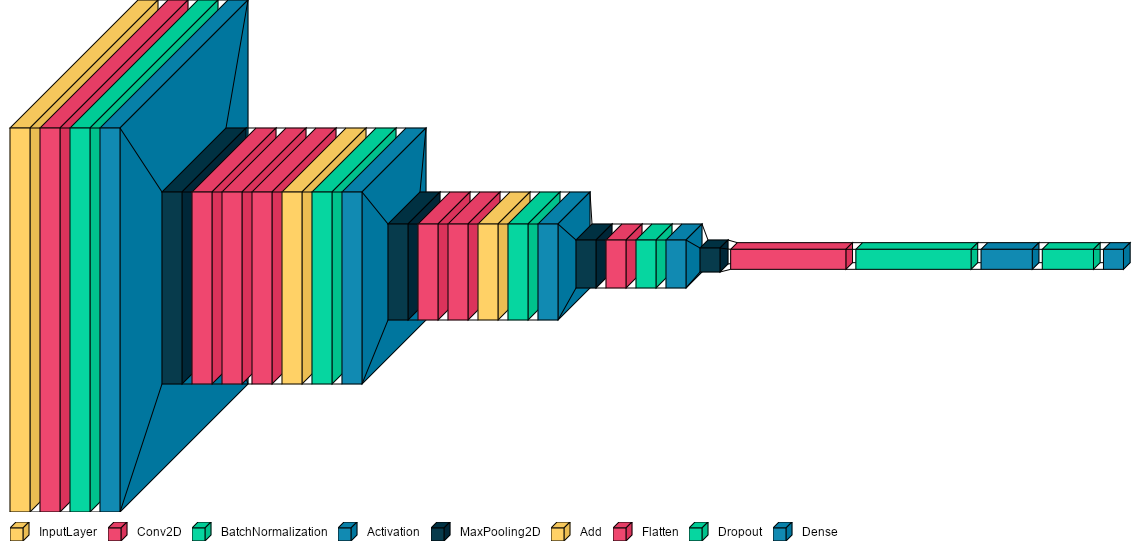
\includegraphics[scale=0.43]{images/soamodel.png}

%---------------------------------------%
\section{Final Model}
ensemble model finale
%---------------------------------------%
\section{Errors and lesson learned}
%---------------------------------------%
\section{Possible improvements}
%---------------------------------------%
\section*{References}
[0] Perez, L., \& Wang, J. (2017). The Effectiveness of Data Augmentation in Image Classification using Deep Learning. arXiv. https://doi.org/10.48550/arXiv.1712.04621\\
{[1]} Mads Dyrmann, Henrik Karstoft, Henrik Skov Midtiby, Plant species classification using deep convolutional neural network, Biosystems Engineering, Volume 151, 2016, Pages 72-80, ISSN 1537-5110 \\
{[2]} Cao, Xudong. "A practical theory for designing very deep convolutional neural networks." Unpublished Technical Report (2015)
\end{document}
